\documentclass[draft=True]{revtex4-2}
\newcommand{\zreco}{\ensuremath{\cos{(\theta_z^{reco})}}}
\newcommand{\ztrue}{\ensuremath{\cos{(\theta_z^{true})}}}
\newcommand{\emm}{\ensuremath{\epsilon_{\mu\mu}}}
\newcommand{\emt}{\ensuremath{\epsilon_{\mu\tau}}}
\newcommand{\eet}{\epsilon_{e\tau}}
\newcommand{\eem}{\epsilon_{e\mu}}
\newcommand{\ett}{\ensuremath{\epsilon_{\tau\tau}}}
\newcommand{\ep}{\ensuremath{\epsilon^\prime}}
\renewcommand{\ne}{\nu_e}
\newcommand{\Ereco}{E^{reco}}
\newcommand{\Etrue}{E^{true}}
\newcommand{\nm}{\nu_\mu}
\newcommand{\nt}{\nu_\tau}
\newcommand{\ane}{\bar\nu_e}
\newcommand{\anm}{\bar\nu_\mu}
\newcommand{\ant}{\bar\nu_\tau}
\newcommand{\dm}{\Delta m^2_{31}}
\newcommand{\sth}{\sin^2(2\theta_{23})}

\usepackage{physics,amsmath, amsfonts, siunitx, amssymb, graphicx, subcaption}
\usepackage[utf8]{inputenc}
\usepackage{hyperref}
\begin{document}
%TODO: nsi intro, clear about factor 3
\section{Detector formalism}
The neutrino flux at the detector is calculated by propagating the atmospheric neutrino flux~\cite{hondapaper} through the Earth by solving the 
Schrödinger equation for varying density. The Earth density profile is taken from the PREM~\cite{PREM}. The baseline for a given trajectory is determined using an average neutrino
production height of 15 km and an Earth radius of 6371 km. %TODO: add more here? no neutrino absorption


The oscillation probability $P_{\alpha \beta}$ acts as a weight to the atmospheric flux, yielding the propagated flux at detector level for flavor $\beta$ as 
\begin{align}\label{eq:propFlux}
    \phi_\beta^\text{det} = \sum_\alpha P_{\alpha\beta} \phi_\alpha^\text{atm} \,,
\end{align}
where we sum over the initial lepton flavors $\alpha \in \{e,\mu, \bar{e}, \bar{\mu}\}$. To illustrate the impact of $\emt$ on both probability
and flux level, we plot the oscillograms resulting from Eq.~\ref{eq:propFlux} in Fig.~\ref{fig:flux_ratio}. In the left panel, we have marked the region in which 99\% of the 
DeepCore cascade events originating from $\ne$ and $\nt$ fluxes are contained. In the right panel, we show the two regions in which 99\% of the IceCube 
and DeepCore track events originating from $\nm$ fluxes are contained. Starting with the $\nm$ flux ratio, we see that the only clear signal discernible to the IceCube detector
is a flux deficiency of a factor of $\sim 10^2$ from core-crossing neutrinos within a zenith range of $\ztrue > -0.87$. DeepCore on the other hand, 
observes multiple fringes of flux surpluses with a factor $\sim 10$. The strongest surplus at \SI{20}{\GeV} is very weakly zenith dependent, a stark contrast to the
energy-independent but zenith-sensetive IceCube deficiency.

For the fluxes which drives cascades, we have to resort to the DeepCore detector alone. %TODO: fill more
Here we see a somewhat weaker signal, this time a zenith-independent deficiency. 
%TODO: fill with conclusion

\begin{figure}[!tb]
   \begin{center}
      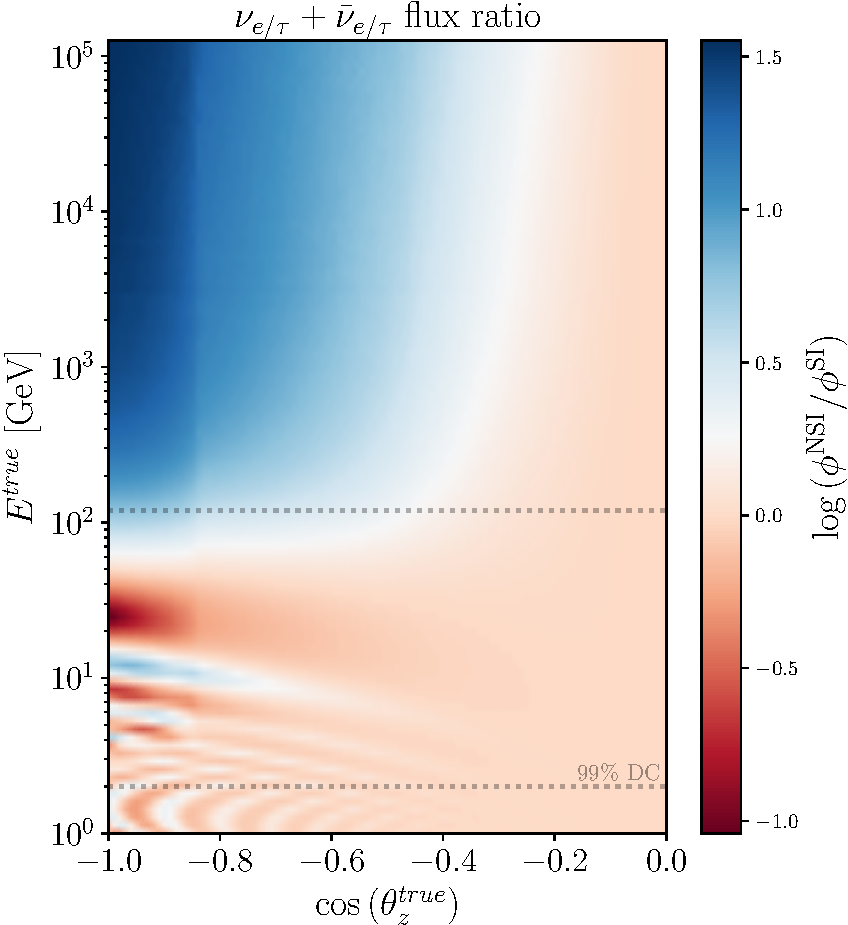
\includegraphics[width=0.35\linewidth]{figures/cascade_flux_ratio.pdf}
      \hspace{1.5cm}
      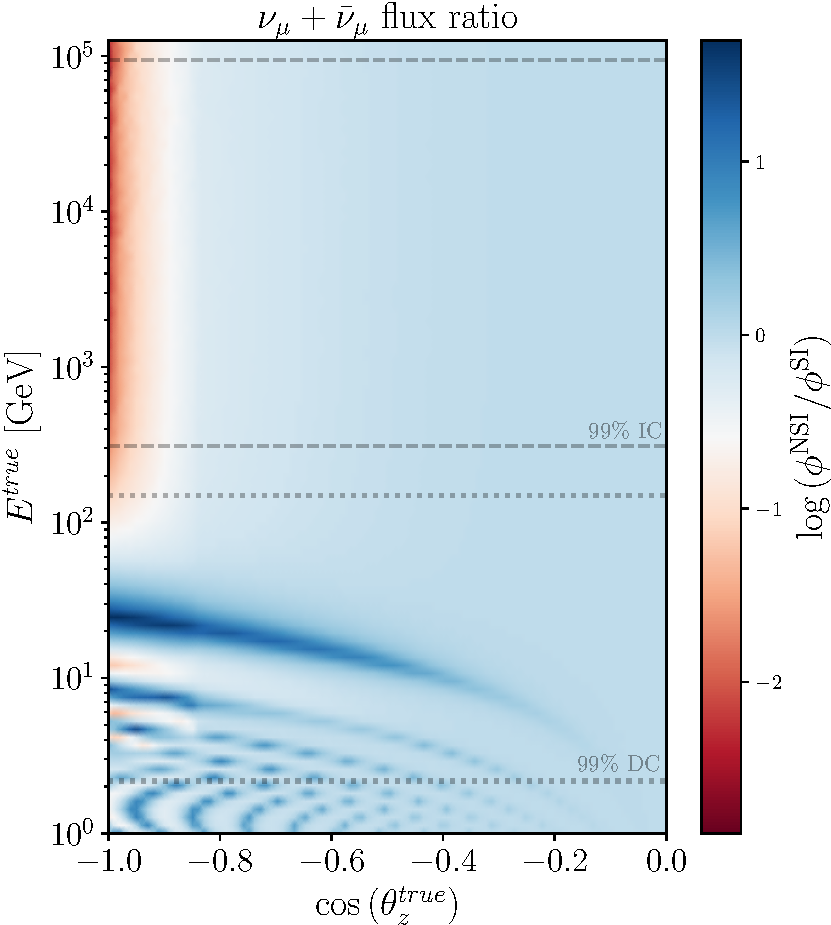
\includegraphics[width=0.35\linewidth]{figures/track_flux_ratio.pdf}
   \end{center}
   \caption{Ratio of propagated NSI to SI atmospheric fluxes at detector level. We set $\emt = -0.05$, and all other NSI parameters to zero. 
   Dotted (dashed) lines show the regions in which 99\% of the 
   DeepCore (IceCube) MC events are contained. \emph{Left panel:} Propagated fluxes of $\ne$ and $\nt$ neutrinos and anti-neutrinos. 
   \emph{Right panel:} Propagated fluxes of $\nm$ neutrinos and anti-neutrinos}\label{fig:flux_ratio}%TODO: normalize color scale and fix limits
\end{figure}% smaller emt and no log. clarify that IC is missing in left panel. clarify
%that energy region within dotted line, use as few words as possible. Normalize color scale. check green-yellow cmap

\subsection{IceCube}\label{ch:ICmethod}
The event rate for each bin reads
\begin{align}\label{eq:ICevents}
   N_{ij} &= T\sum_\beta \int_{(\cos{\theta_z^r})_i}^{(\cos{\theta_z^r})_{i+1}} \dd \cos{\theta^r_z} \int_{E^r_{j}}^{E^r_{j+1}} \dd E^r \int_0^\pi R(\theta^r,\theta^t) \dd \cos{\theta^t} \int_0^\infty \phi_\beta^\text{det}  A^\text{eff} R(E^r,E^t) 
   \dd E^t\,,
\end{align}
where $T$ is the live time of the detector, and $A^\text{eff}$ its effective area averaged over the flavors $\beta$ from~\cite{ICaeff}. $R(x^r,x^t)$ is a resolution function, 
which is responsible for the smearing between the reconstructed and true parameters $x^r$ and $x^t$, respectively. We assume a log-normal distribution, giving it the form 
\begin{align}
    R(x^r, x^t) = \frac{1}{\sqrt{2\pi} \sigma_{x^r}x^r} \exp\left[-\frac{(\log x^r-\mu(x^t))^2}{2\sigma_{x^r}^2}\right]\,.
\end{align}
As seen in Fig.~\ref{fig:IC_MC_counts}, the energy reconstruction is biased. To model this relationship between $\Etrue$ and $\Ereco$, we train a Gaussian process regressor on the dataset~\cite{IC2016}, from which
we can extract a predicted mean and standard deviation for a given $E^{reco}$. We then take the $\Etrue$ points of the 99th percentile of each distribution to obtain
the limits of $\Etrue$ at which to integrate over. We have no angular resolution function since the angle resolution in IceCube for track-like events is less than $\SI{2}{\degree}$, making $\ztrue$ coincide with $\zreco$ for our study. 
The data is from the 86 string sterile analysis~\cite{IC2020}.

\subsection{DeepCore}\label{ch:DCmethod}
In this part, we use the publically available DeepCore data sample~\cite{DC2019data} which is an updated version of what was used by the 
IceCube collaboration in a $\nu_\mu$ disapprearance analysis~\cite{DC2018mudisappearance}.

The detector systematics include ice absorption and scattering, and overall, lateral, and head-on optical efficiencies of the DOMs. 
They are applied as correction factors using the best-fit points from the DeepCore 2019 $\nu_\tau$ appearance 
analysis~\cite{DC2019tauappearance}.

The data include 14901 track-like events and 26001 cascade-like events, both divided into eight 
$ \log_{10}E^{reco} \in [0.75,1.75]$ bins, and eight $\zreco \in [-1,1]$ bins. Each event has a Monte Carlo weight $w_{ijk,\beta}$,
from which we can construct the event count as
\begin{align}\label{eq:MCevents}
    N_{ijk} &= C_{ijk}\sum_{\beta}w_{ijk,\beta}\, \phi_\beta^\text{det}\,,
\end{align}
where $C_{k\beta}$ is the correction factor from the detector systematic uncertainty and $\phi_\beta^\text{det}$ is defined as Eq.~\ref{eq:propFlux}. We have now substituted the effect of the Gaussian smearing 
by treating the reconstructed and true quantities as a migration matrix. 

The oscillation parameters used on our DeepCore simulations are from the
best-fit in the global analysis in~\cite{nufit}: $\theta_{12} = \SI{33.44}{\degree},\, \theta_{13} = \SI{8.57}{\degree},\, \Delta m^2_{21} =  \SI{7.42}{\electronvolt^2}$, and we 
marginalize over $\dm$ and $\theta_{23}$.

We plot the event pull $(N_{NSI} - N_{SI})/\sqrt{N_{SI}}$ where $N_{SI}$ $(N_{NSI})$ are the numbers of expected events
assuming standard (non-standard) interactions in Fig.~\ref{fig:DC_event_pulls}. This gives the normalized difference in the
number of expected events at the detector, and illustrates the expected sensitivity of DeepCore for the NSI parameters.

\begin{figure}[t]
   \begin{center}
         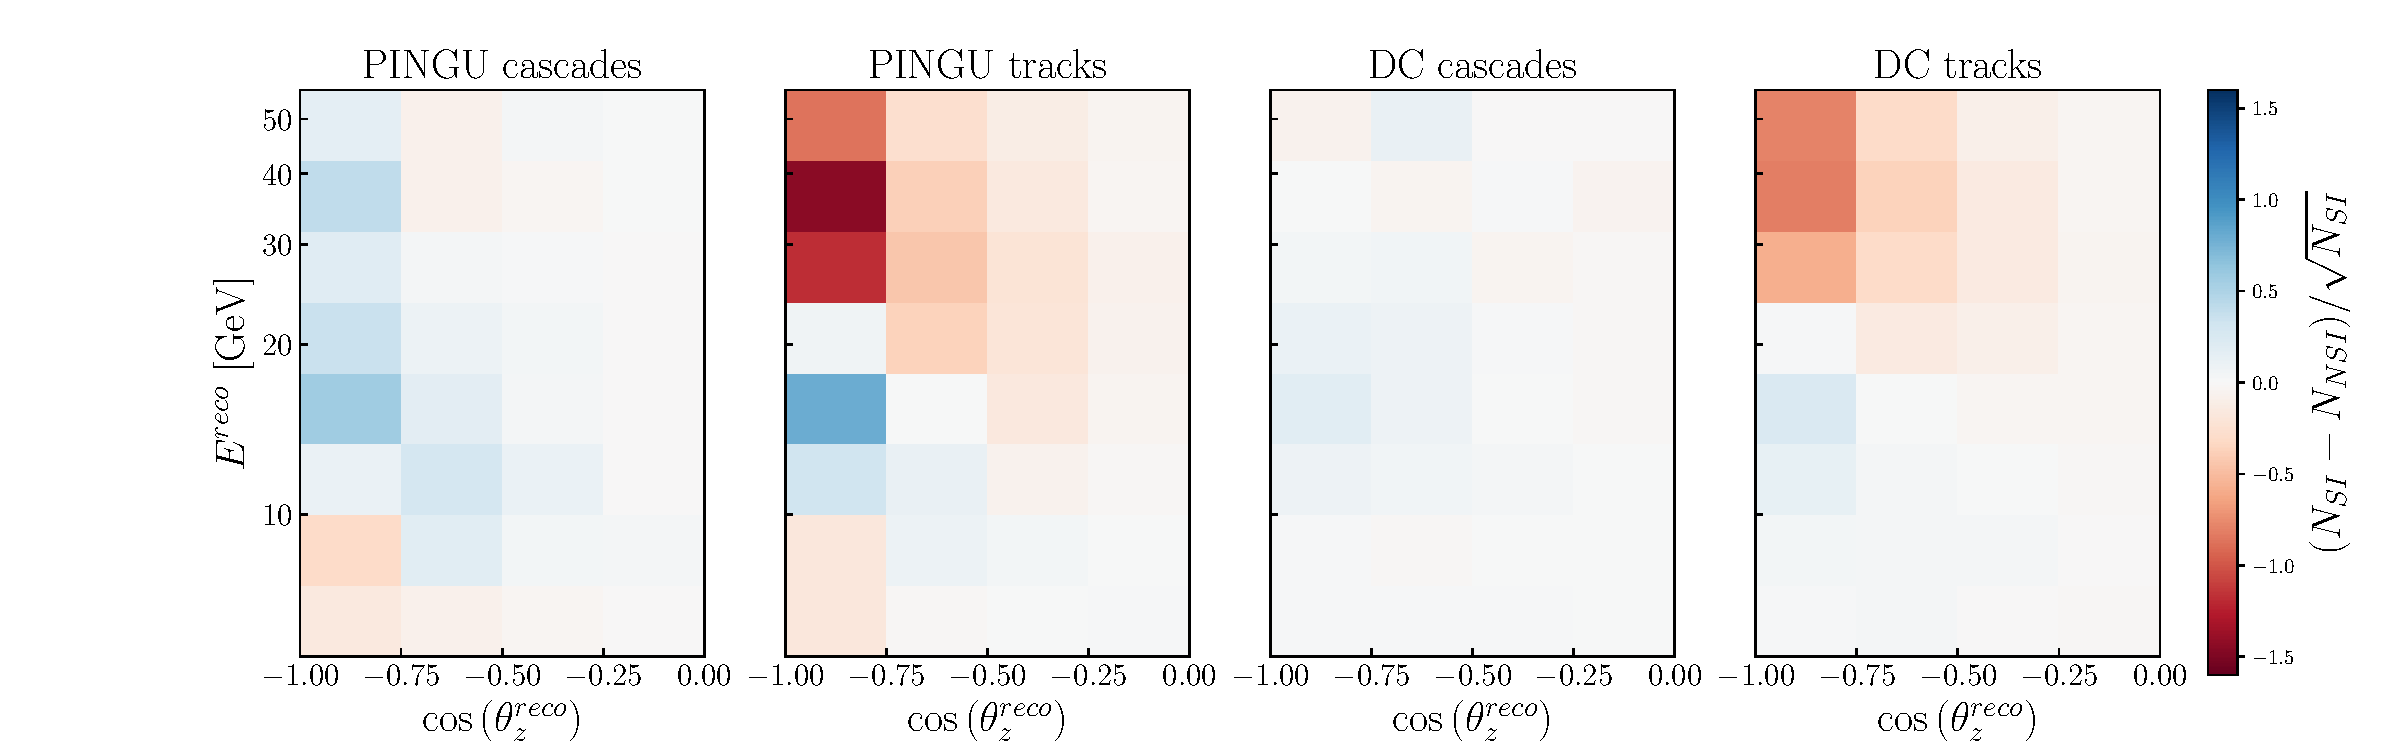
\includegraphics[width=0.9\textwidth]{figures/event_pulls.pdf}
   \end{center}
   \caption{Expected pulls of the form $(N_{NSI} - N_{SI})/\sqrt{N_{SI}}$ for PINGU and DeepCore after 3 years. We compare the NSI event count with $\emt=-0.01$
    to the standard interaction count}\label{fig:event_pulls} 
\end{figure}


\subsection{PINGU}\label{ch:PINGUmethod}
The methodology behind the PINGU simulations are the same as with our DeepCore study~\ref{ch:DCmethod}. We use the public MC~\cite{PINGUdata}, which allows us to construct the event count as in Eq.~\ref{eq:MCevents}.
However, since no detector systematics is yet modelled for PINGU, the correction factors $C_{ijk}$ are all unity.
As with the DeepCore data, the PINGU MC is divided into eight 
$\log_{10}E^{reco} \in [0.75,1.75]$ bins, and eight $\zreco \in [-1,1]$ bins for both track- and cascade-like events. Just as with DeepCore, 
we plot the events pulls for cascades and tracks in Fig.~\ref{fig:PINGU_event_pulls}. %TODO:talk about this
We generate `data' by predicting the event rates at PINGU with the following best-fit parameters from~\cite{nufit}, except for the CP-violating phase which is set to zero for simplicity.

\begin{align}\label{eq:PINGUparams}
    &\Delta m^2_{21} =  \SI{7.42e-5}{\electronvolt^2},\hspace{0.5em} \dm =  \SI{2.517e-3}{\electronvolt^2}, \nonumber \\
    &\theta_{12} = \SI{33.44}{\degree},\hspace{1em} \theta_{13} = \SI{8.57}{\degree},\hspace{1em} \theta_{23} = \SI{49.2}{\degree}, \hspace{1em} \delta_\text{CP} = 0\,.
\end{align}


\section{Results}
%Short intro
\subsection{Methodology}
For our analyses, we define our $\chi^2$ as
\begin{align} \label{eq:chisq}
    \chi^{2}(\hat{\theta},\alpha,\beta, \kappa)=\sum_{ijk} \frac{\left(N^\text{th}-N^\text{data}\right)_{ijk}^{2}}
    {\left(\sigma^\text{data}_{ijk}\right)^{2} + \left(\sigma^\text{syst}_{ijk}\right)^{2}}+ 
    \frac{(1-\alpha)^2}{\sigma_\alpha^2} + \frac{\beta^2}{\sigma_\beta^2}\,
\end{align}
where we minimize over the model parameters $\hat{\theta} \in \{\dm, \theta_{23}, \epsilon\}$, the penalty terms $\alpha$ and $\beta$, and the free parameter $\kappa$.
$N_{ijk}^\text{th}$ is the expected number of events from theory, and $N_{ijk}^\text{data}$ is the observed number of events in that bin. We set $\sigma_\alpha = 0.25$ as the atmospheric flux normalization error, and $\sigma_\beta = 0.04$ as the zenith angle slope error~\cite{hondapaper}. 
The observed event number has an associated Poissonian uncertainty $\sigma_{ijk}^\text{data} = \sqrt{N_{ijk}^\text{data}}$.
% Make clear distinction of different sigma syst here.
For IceCube, the event count takes the form
\begin{align}
    N^\text{th}_{ijk} = \alpha\left[1+\beta (0.5 + \zreco_i )\right] N_{ijk}(\hat{\theta})\,,
\end{align}
with $N_{ijk}(\hat{\theta})$ from Eq.~\ref{eq:ICevents}. Here, we allow the event distribution to rotate around the median zenith angle of $\zreco = -0.5$.

For DeepCore and PINGU, and the event count takes the form
\begin{align}
    N^\text{th}_{ijk} = \alpha\left[1+\beta \zreco_i \right] N_{ijk}(\hat{\theta}) + \kappa N_{ijk}^{\mu_{atm}}\,,
\end{align}
with $N_{ijk}(\hat{\theta})$ from Eq.~\ref{eq:MCevents}. $N_{ijk}^{\mu_{atm}}$ is the muon background, which is left to float freely in the DeepCore analysis.
The background at PINGU can be considered neglible to first order~\cite{PINGUdata}, and we thus put $\kappa=0$ when calculating the PINGU $\chi^2$\,. 
Since the median zenith is $\zreco = 0$ for DeepCore and PINGU, we allow the event count to rotate around zero.
For IceCube, we set $\sigma_{ijk}^\text{syst} = f\sqrt{N_{ijk}^\text{data}}$. %TODO: and take ... %.
For DeepCore, we use the provided systematic error distribution which accounts for both uncertanties in the finite MC statistics and in the data-driven 
muon background estimate~\cite{DC2019data}. %TODO segue

\subsection{Constraining the NSI parameters}
First, we set all standard oscillation parameters to their current best-fit values of Eq.~\ref{eq:PINGUparams}, except for $\dm$ and $\theta_{23}$, 
which we marginalize over their $3\sigma$ ranges of \SI{2.435e-3} to \SI{2.598e-3}{\electronvolt^2} and \SI{40.1} to \SI{51.7}{\degree} respectively. %TODO: make unit ranges nicer.
After the oscillation parameters have been marginalized out, we plot $\Delta \chi^2$ for each of the four NSI parameters in Fig.~\ref{fig:3D_NO}. We record the 
confidence levels in Table.~\ref{table:DC_PINGU_results} and best-fit points in Table ~\ref{table:bestfit}.

\begin{figure}[!tb]
   \begin{center}
      \begin{subfigure}{0.4\textwidth}
         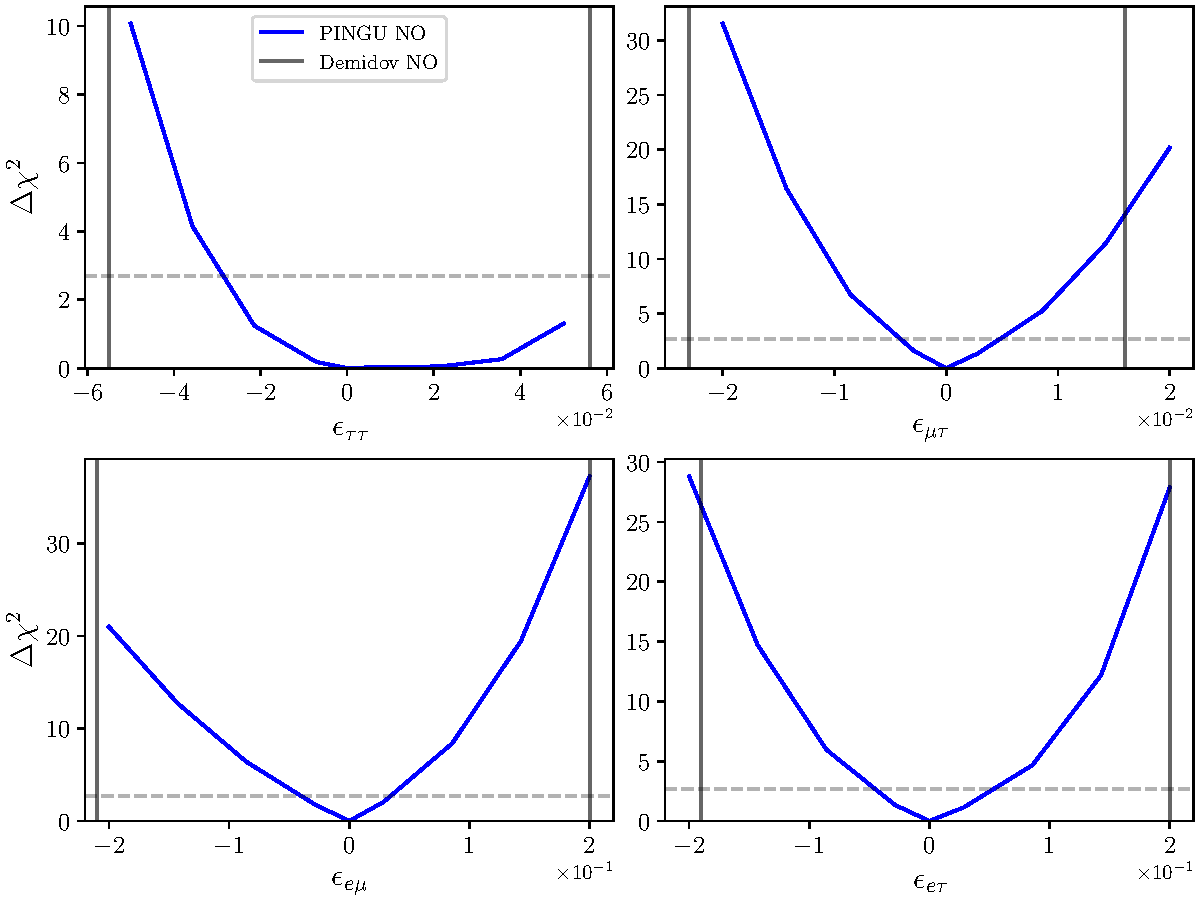
\includegraphics[width=1\linewidth]{figures/PINGU_3D_NO.pdf}
         \caption{PINGU}\label{fig:PINGU_3D_NO}
      \end{subfigure}
      \hspace{1cm}
      \begin{subfigure}{0.4\textwidth}
         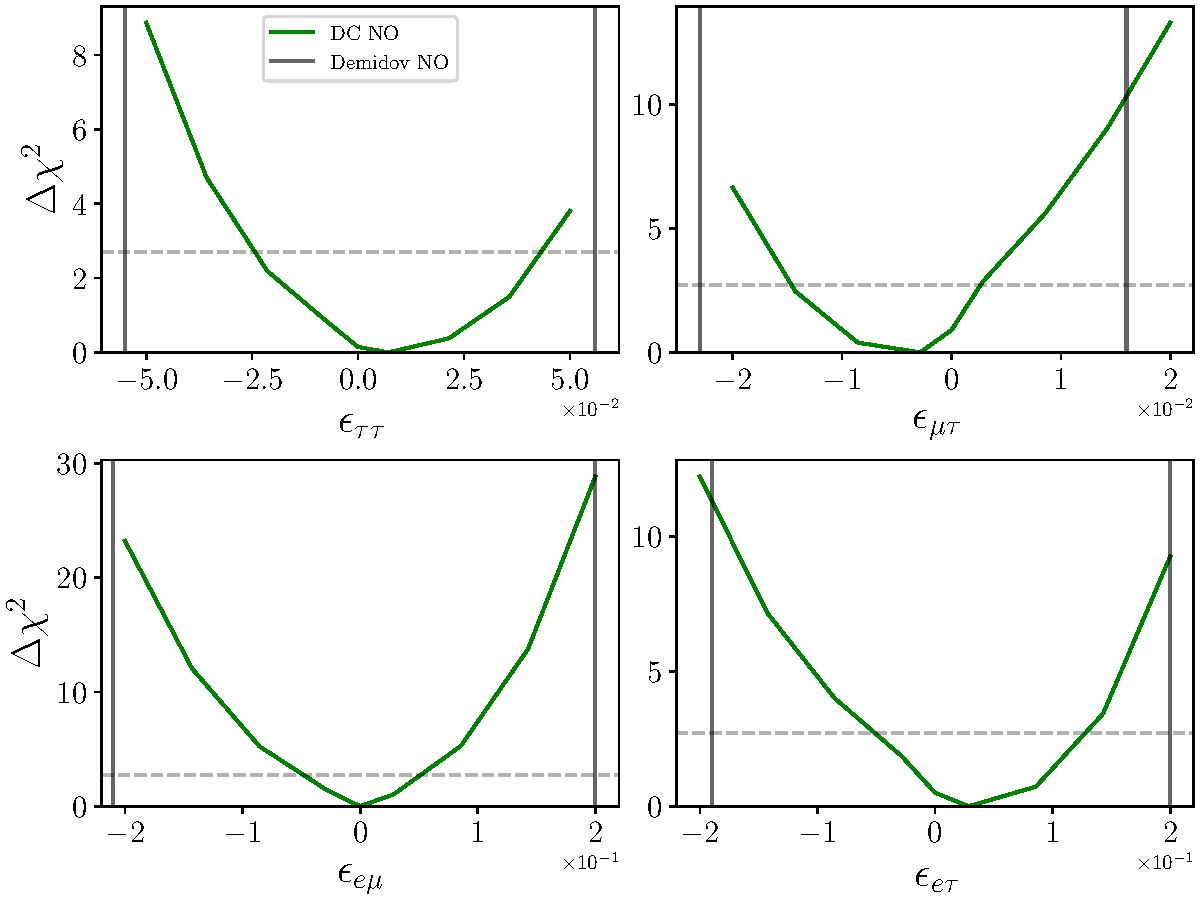
\includegraphics[width=1\linewidth]{figures/DC_3D_NO.pdf}
         \caption{DeepCore}\label{fig:DC_3D_NO}
      \end{subfigure}
    \end{center}
    \caption{Minimization of the $\Delta \chi^2$ defined in Eq.~\ref{eq:chisq} after three years of data.
    $\dm$ and $\theta_{23}$ and have been marginalized out, and all other NSI 
    parameters other than the one shown in each panel are fixed to zero.}\label{fig:3D_NO}
 \end{figure}
%TODO:explain emt assymetry. dont put pingu and dc side by side since pingu is generated.. include 3sigma if possible?
%TODO: ploit contour for ett-emt
 \begin{table}
   \begin{center}
   \begin{tabular}{lcc}
           \hline \hline \\
           Parameter & 90\% CL & $3\sigma$  \\
           \hline \multicolumn{3}{c} {\hspace{1.5cm} DeepCore }  \\[0.1em]
           $\ett$ & [-0.029, 0.044]\hspace{1cm} & [-, -] \\
           $\emt$ & [-0.015, 0.005]\hspace{1cm} & [-, 0.015] \\
           $\eem$ & [-0.072, 0.075]\hspace{1cm} & [-0.132, 0.127]\\
           $\eet$ & [-0.074, 0.141]\hspace{1cm} & [-0.174, 0.2  ]\\\\
           \multicolumn{3}{c} {\hspace{1.5cm} PINGU } \\
           $\ett$ & [-0.033, -]\hspace{1cm} & [-0.048, -] \\
           $\emt$ & [-0.007, 0.007]\hspace{1cm} & [-0.011, 0.013] \\
           $\eem$ & [-0.062, 0.057]\hspace{1cm} & [-0.122, 0.103] \\
           $\eet$ & [-0.069, 0.077]\hspace{1cm} & [-0.121, 0.133] \\\\
           \multicolumn{3}{c} {\hspace{1.5cm} DeepCore + PINGU } \\
           $\ett$ & [-0.028, 0.043]\hspace{1cm} & [-0.043, -]\\
           $\emt$ & [-0.007, 0.005]\hspace{1cm} & [-0.011, 0.01] \\
           $\eem$ & [-0.048, 0.048] \hspace{1cm} & [-0.09, 0.085]\\
           $\eet$ & [-0.054, 0.072] \hspace{1cm} & [-0.101, 0.118] \\
           \hline
           \hline
   \end{tabular}
   \end{center}
   \caption{DeepCore and PINGU results from the $\Delta \chi^2$ in Fig.~\ref{fig:3D_NO}.}\label{table:DC_PINGU_results}
\end{table}

\begin{table}
   \begin{center}
   \begin{tabular}{lccc}
           \hline \hline & \multicolumn{3}{c} {\text {Best fit}} \\
           \cline { 2 - 4 } Parameter & $\dm$ & $\theta_{23}$  & $\epsilon$  \\
           \hline \multicolumn{3}{c} {\hspace{2.5cm} DeepCore }  \\[0.1em]
           $\ett$ &  2.435 & 47.84 & 0.0125 \\
           $\emt$ &  2.435 & 43.97 & -0.005 \\
           $\eem$ &  2.435 & 43.97 & 0 \\
           $\eet$ &  2.435 & 43.97  & 0.05 \\\\
           \multicolumn{3}{c} {\hspace{2.5cm} IceCube } \\
           $\emt$ &  - & - & - \\
           \hline
           \hline
   \end{tabular}
   \end{center}
   \caption{Best fit points for $\dm$ and $\theta_{23}$ are given in units of $\si{10^{-3}\eV\squared}$ and
   degrees, respectively.}\label{table:bestfit}
\end{table}
%TODO:  include ranges for different f.
%make log table with secyions of dc, p, ic, dc+p
Comparing the PINGU results in Fig.~\ref{fig:PINGU_3D_NO} and the DeepCore results in Fig.~\ref{fig:DC_3D_NO}, we note that 
the best-fit for each NSI parameter for the PINGU experiment is expected to be zero. This is because the `data' we generated during 
the PINGU simulations assumes no NSI since they have yet to be observed in nature. This introduces a non-NSI bias in our joint analysis,
since PINGU has stronger statistics than DeepCore, and will thus pull the joint $\chi^2$ towards $\epsilon =0$.

%TODO: segue to joint
For the joint analysis, we follow the parameter goodness-of-fit prescription~\cite{maltoni2003} and construct the joint $\chi^2$ as 
\begin{align}\label{eq:joint_chisq}
    \chi^2_\text{joint} = \chi^2_\text{IC} + \chi^2_\text{DC} + \chi^2_\text{P} - \chi^2_{IC,min} - \chi^2_\text{DC,min} - \chi^2_\text{P,min}\,
\end{align}
with test statistic $\chi^2_\text{joint,min}$. The results are shown in Fig.~\ref{fig:joint_3D} and summarized in Table~\ref{table:DC_PINGU_results}.

\begin{figure}[t]
    \begin{center}
       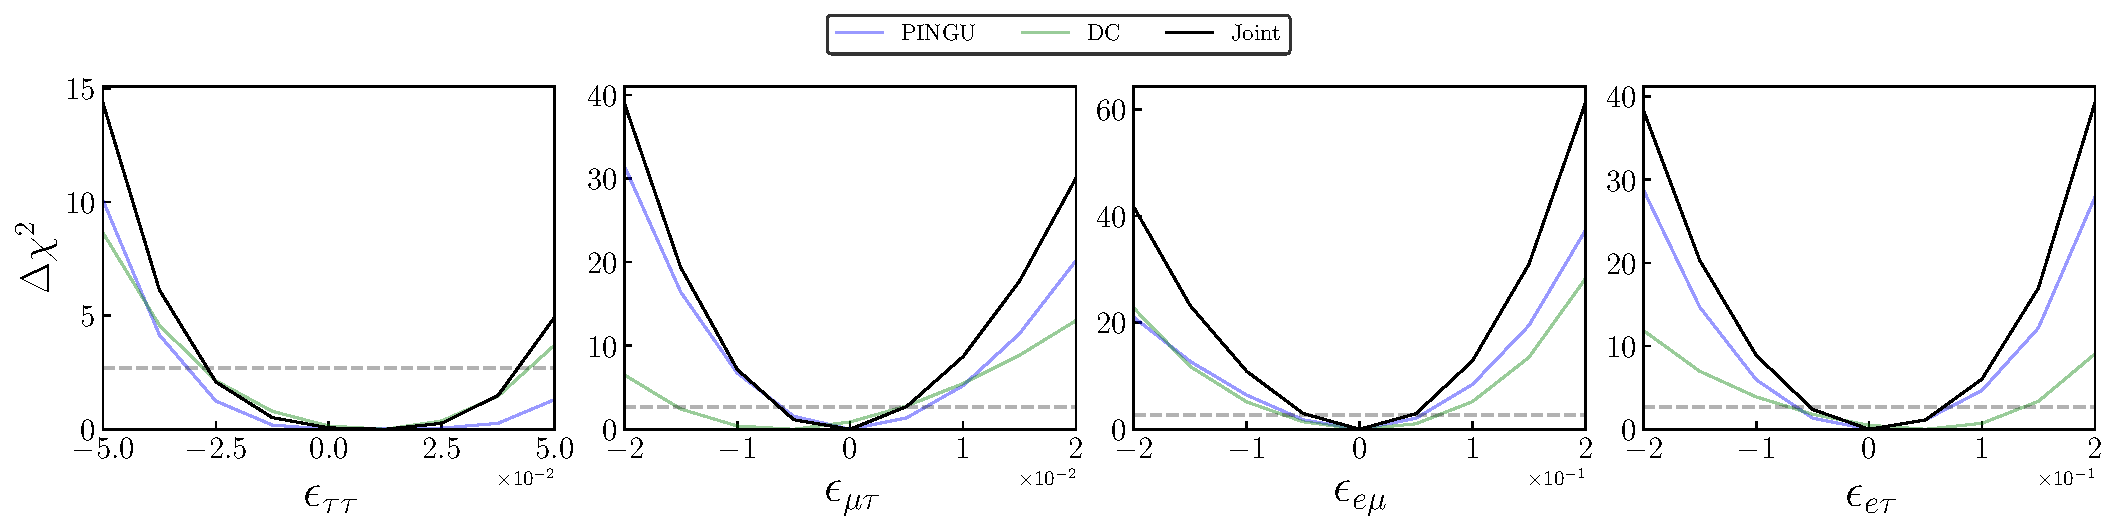
\includegraphics[width=0.9\linewidth]{figures/joint_3D_NO.pdf}
    \end{center}
    \caption{Expected joint $\Delta \chi^2$ from Eq.~\ref{eq:joint_chisq} for normal ordering.}
    \label{fig:joint_3D}
 \end{figure}


%TODO:  Discussion on impact of IC on chisq.?

%TODO: subsection about comparison between different papers. 
\bibliographystyle{elsarticle-num}
\bibliography{article}

\newpage
\begin{tabular}{p{55mm}p{55mm}p{55mm}}
   DeepCore (2017)
      \begin{itemize}
         \item[$\checkmark$] Honda atmospheric fluxes
         \item[$\times$] Only look at tracks and $\emt$
         \vspace{1em}  
         \item[$\times$] DC Monte Carlo from an older dataset 
         \item[$\times$] 8 E bins from $\SI{6.3}{\electronvolt^2}$ to $\SI{56}{\electronvolt^2}$
         \item[$\times$] 8 z bins from -1 to 0 
         \item[$\times$] Use "Overall" and "relative $\ne$ to $\nm$" normalization
         \item[$\times$] Prior on spectral index
         \item[$\times$] No zenith angle normalization
         \item[$\checkmark$] No priors on $\dm, \theta_{23},\theta_{13}$
      \end{itemize} &
    Demidov (2020) DC analysis
      \begin{itemize}
         \item[$\checkmark$] Honda atmospheric fluxes
         \item[$\checkmark$] Looks at tracks + cascades for $\emt$ and $\ett$
         \item[$\checkmark$] Data and Monte Carlo from DC 2018
         \item[$\checkmark$] 8 E bins from $\SI{5.6}{\electronvolt^2}   $ to $\SI{56}{\electronvolt^2}$
         \item[$\checkmark$] 8 z bins from -1 to 1
         \item[$\times$] Use "Overall" and "relative $\ne$ to $\nm$" normalization
         \item[$\times$] Prior on spectral index
         \item[$\times$] No zenith angle normalization
         \item[$\checkmark$] No priors on $\dm, \theta_{23}$
         \item[$\checkmark$] Fixes $\Delta m^2_{21}, \theta_{12}, \theta_{13}$
         \item[$\times$] Uncertainty on hadron production in atmosphere
         \item[$\times$] Uncertainty on neutrino nucleon cross section 
      \end{itemize} &
    This DC+PINGU analysis
      \begin{itemize}
         \item[$\checkmark$] Honda atmospheric fluxes
         \item[$\checkmark$] Tracks and cascades for all flavors
         \vspace{1em} 
         \item[$\checkmark$] Reco $\to$ true mapping from Monte Carlo migration matrix
         \item[$\checkmark$] 8 E bins from $\SI{5.6}{\electronvolt^2}$ to $\SI{56}{\electronvolt^2}$
         \item[$\checkmark$] 8 zenith angle bins from -1 to 1
         \item[$\checkmark$] Flux normalization uncertainty of 25\%
         \item[$\checkmark$] Zenith angle uncertainty of 4\% 
         \item[$\checkmark$] No priors on oscillation parameters 
         \item[$\checkmark$] Marginalize $\dm$ and $\theta_{23}$. All other oscillation parameters are fixed.
      \end{itemize} 
\end{tabular}
\end{document}


